\chapter{One-loop neutrino masses}
Here we calculate the one-loop neutrino mases in the mass-basis


\section{Extra particles}
We assume to have $\alpha$-scalar  and $n$-fermions in the mass eigenstate basis in Weyl spinor notation
\begin{align}
  \mathcal{L}=\left(y_{in\alpha}\nu_{i}\chi_n S_{\alpha}+m_n \chi_n\chi_n +\text{h.c} \right)+\tfrac{1}{2}m_{\alpha}^2\,S_{\alpha}^2\,.
\end{align}
From left to right (clockwise) in Figure~\ref{fig:1lnu}
\begin{figure}
  \centering
  \includegraphics[scale=0.5]{onelooopneutrino}
  \caption{Generic one-loop neutrino mass contribution}
  \label{fig:1lnu}
\end{figure}

\begin{align}
-i\Sigma^{\nu}_{ij}(p)=&\int \frac{d4k}{\left( 2\pi \right)^{4}}\left(y_{in\alpha}  \right)iS_F(k) \left(y_{jn\alpha}\right)i\Delta_F(p+k) \nonumber\\
=&\frac{y_{i n\alpha}y_{j n\alpha}}{16\pi^2}\int \frac{d^4k}{i\pi^2}\frac{\cancel{k}+m_{\chi_n}}{\left(k^2-m_{\chi_n}^2  \right)\left[\left(p+k\right)^2-m_{S_\alpha}^2\right]}
\end{align}

In the limit $p\to 0$
\begin{align}
\label{eq:mnub0}
   M^{\nu}_{ij}=&-\frac{y_{i n\alpha}y_{j n\alpha}}{16\pi^2}m_{\chi_n} B_0 \left( 0;m_{\chi_n}^2,m_{S_{\alpha}}^2 \right) \,.
\end{align}
where $B_0\left
(0;m_{\chi_n}^2,m^2_{S_{\alpha}} \right)$ is the $B_0$ Passarino-Veltman function~\cite{Passarino:1978jh} in dimensional regularization 

\begin{align}
  \label{eq:mnueigi02}
  B_0 \left(0;m_{\chi_n}^2,m^2_{S_{\alpha}} \right)=&\frac{\left( 2\pi \mu \right)^{\epsilon}}{i\pi^2}\int d^dk\frac{1}{\left(k^2-m_{\chi_n}^2\right)\left(k^2-m_{S_\alpha}^2\right)}\,.
\end{align}
where $\mu$ is the subtraction point of dimensional regularization and $d=4-\epsilon$.

By following Romao notes: \url{http://porthos.tecnico.ulisboa.pt/Public/textos/one-loop.pdf}\footnote{Old version, now is a part of "Advanced Quantum Field Theory" \url{http://porthos.ist.utl.pt/Public/textos/tca.pdf}} 
it will be shown below that this can be decomposed as
\begin{align}
  \label{eq:mnueig}
  B_0 \left(0;m_{\chi_n}^2,m^2_{S_{\alpha}} \right)
            =&\frac{1}{m_{\chi_n}^2-m_{S_\alpha}^2}\left[ A_0\left(m_{\chi_n}^2\right)-A_0\left(m_{S_\alpha}^2\right)  \right],
\end{align}
where
\begin{align}
   A_{0}\left(m^{2}\right) &=\frac{(2 \pi \mu)^{\epsilon}}{i \pi^{2}} \int d^{d} k \frac{1}{k^{2}-m^{2}}\,.
\end{align}


To evaluate the integral through the Passarino-Veltman functions, we start with the general integral with two denominators
\begin{align}
  \label{eq:pvbo}
  B_{0}\left(r_{10}^{2}, m_{0}^{2}, m_{1}^{2}\right)=\frac{(2 \pi \mu)^{\epsilon}}{i \pi^{2}} \int d^{d} k \prod_{i=0}^{1} \frac{1}{\left[\left(k+r_{i}\right)^{2}-m_{i}^{2}\right]}
\end{align}
In particular

\begin{align}
  I =&\int \frac{d^{d} k}{(2 \pi)^{d}} \frac{1}{\left[(k+p)^{2}-m_{1}^{2}+i \epsilon\right]\left[k^{2}-m_{2}^{2}+i \epsilon\right]} \nonumber\\
    =&\int_{0}^{1} d x \int \frac{d^{d} k}{(2 \pi)^{d}} \frac{1}{\left[k^{2}+2 p \cdot k x+p^{2} x-m_{1}^{2} x-m_{2}^{2}(1-x)+i \epsilon\right]^{2}} \nonumber\\
  =&\int_{0}^{1} d x \int \frac{d^{d} k}{(2 \pi)^{d}} \frac{1}{\left[k^{2}+2 P(x) \cdot k-M^{2}(x)+i \epsilon\right]^{2}} \nonumber\\
  =&\int_{0}^{1} d x \int \frac{d^{d} k}{(2 \pi)^{d}} \frac{1}{\left\{[k+P(x)]^{2}-P^{2}(x)-M^{2}(x)+i \epsilon\right\}^{2}}
\end{align}
where
\begin{align}
  P(x)=&x p\,,& M^{2}(x)=&-x p^{2}+m_{1}^{2} x+m_{2}^{2}(1-x).
\end{align}
Changing variable $k\to k-P$
\begin{align}
  I=\int_{0}^{1} d x \int \frac{d^{d} k}{(2 \pi)^{d}} \frac{1}{\left[k^{2}-C(x)+i \epsilon\right]^{2}}
\end{align}
where
\begin{align}
  \label{eq:cx}
  C(x)=P^{2}(x)+M^{2}(x)
\end{align}


In general, the integral to be calculated with dimensional regularization is
\begin{align}
  I_{r, m}=\int \frac{d^{d} k}{(2 \pi)^{d}} \frac{k^{2^{r}}}{\left[k^{2}-C+i \epsilon\right]^{m}}\,.
\end{align}
Making a Wick rotation, this can be written as
\begin{align}
  I_{r, m}=i(-1)^{r-m} \int \frac{d^{d} k_{E}}{(2 \pi)^{d}} \frac{k_{E}^{2^{r}}}{\left[k_{E}^{2}+C\right]^{m}}
\end{align}
where $k_{E}=\left(k_{E}^{0}, \boldsymbol{k}\right)$ is an euclidean vector with
\begin{align}
  k^{0}=&i k_{E}^{0}\,,& \text{and} && k_{E}^{2}=&\left(k_{E}^{0}\right)^{2}+|\boldsymbol{k}|^{2}\,.
\end{align}


The integral can be evaluated to give
\begin{align}
  I_{r, m}=i C^{r-m+\frac{d}{2}} \frac{(-1)^{r-m}}{(4 \pi)^{\frac{d}{2}}} \frac{\Gamma\left(r+\frac{d}{2}\right)}{\Gamma\left(\frac{d}{2}\right)} \frac{\Gamma\left(m-r-\frac{d}{2}\right)}{\Gamma(m)}\,.
\end{align}
By using $d=4-\epsilon$
\begin{align}
  I_{r, m}=i \frac{(-1)^{r-m}}{(4 \pi)^{2}}\left(\frac{4 \pi}{C}\right)^{\frac{\epsilon}{2}} C^{2+r-m} \frac{\Gamma\left(2+r-\frac{\epsilon}{2}\right)}{\Gamma\left(2-\frac{\epsilon}{2}\right)} \frac{\Gamma\left(m-r-2+\frac{\epsilon}{2}\right)}{\Gamma(m)}\,.
\end{align}

We are interested in
\begin{align}
  I_{0,2}=\frac{i}{(4 \pi)^{2}}\left(\frac{4 \pi}{C}\right)^{\frac{\epsilon}{2}} \Gamma\left(\frac{\epsilon}{2}\right).
\end{align}
where
\begin{align}
  \Gamma\left(\frac{\epsilon}{2}\right)=\frac{2}{\epsilon}+\psi(1)+O(\epsilon)
\end{align}
where
\begin{align}
\psi(z) &=\frac{d}{d z} \ln \Gamma(z) \\ \psi(1) &=-\gamma \,.
\end{align}

So that
\begin{align}
  I_{0,2}=\frac{i}{16 \pi^{2}}\left(\Delta_{\epsilon}-\ln C\right)
\end{align}
where
\begin{align}
  \Delta_{\epsilon}=\frac{2}{\epsilon}-\gamma+\ln 4 \pi\,,
\end{align}
where $\gamma$ is the Euler-Mascheroni constant.


Replacing back $C(x)$ from eq~\eqref{eq:cx} in \eqref{eq:pvbo}

\begin{align}
  \label{eq:gpvbo}
  B_{0}\left(p^{2}, m_{0}^{2}, m_{1}^{2}\right)=\Delta_{\epsilon}-\int_{0}^{1} d x \ln \left[\frac{-x(1-x) p^{2}+x m_{1}^{2}+(1-x) m_{0}^{2}}{\mu^{2}}\right]
\end{align}

\begin{verbatim}
In[1]:= Integrate[Log[a x], x]
Out[1]= -x + x Log[a x]


In[2]:= Dt[-x + x Log[a x], x, Constants -> a]
Out[3]= Log[a x]
\end{verbatim}

Taking into account that

\begin{align}
  \label{eq:I01}
  I_{0,1}=\frac{i}{16 \pi^{2}} C\left(1+\Delta_{\epsilon}-\ln C\right)\,,
\end{align}
we can define
\begin{align}
   A_{0}\left(m^{2}\right) &=\frac{(2 \pi \mu)^{\epsilon}}{i \pi^{2}} \int d^{d} k \frac{1}{k^{2}-m^{2}}\,.
\end{align}
such that
\begin{align*}
  A_0\left(m^2\right)=m^2 \left[ \Delta_{\epsilon}+1-\ln \left( m^2/\mu^2 \right) \right]
\end{align*}

In this way, from \eqref{eq:gpvbo} we can get
\begin{align}
  B_{0}\left(0, m_{0}^{2}, m_{1}^{2}\right)=&\Delta_{\epsilon}+1-\frac{m_{0}^{2} \ln \frac{m_{0}^{2}}{\mu^{2}}-m_{1}^{2} \ln \frac{m_{1}^{2}}{\mu^{2}}}{m_{0}^{2}-m_{1}^{2}} \nonumber\\
 =&\frac{A_{0}\left(m_{0}^{2}\right)-A_{0}\left(m_{1}^{2}\right)}{m_{0}^{2}-m_{1}^{2}}\,.
\end{align}


Replacing back in eq.~\eqref{eq:mnueig}, we have
\begin{align}
   B_0 \left(0;m_{\chi_n}^2,m^2_{S_{\alpha}} \right)=&
   \frac{1}{m_{\chi_n}^2-m_{S_\alpha}^2}\left[m^2_{\chi_n} \left[ \Delta+1-\ln \left( m_{\chi_n}^2/\mu^2 \right) \right]  \right] 
-m_{S_\alpha}^2 \left[ \Delta+1-\ln \left( m_{S_\alpha}^2/\mu^2 \right) \right] \nonumber\\
  =&(\Delta+1)+\frac{m_{S_\alpha}^2\ln \left( m_{S_\alpha}^2/\mu^2 \right)-m_{\chi_n}^2\ln \left( m_{\chi_n}^2/\mu^2 \right)}{m_{\chi_n}^2-m_{S_\alpha}^2} \nonumber\\
 =&(\Delta+1)+\frac{m_{S_\alpha}^2 \left[ \ln \left( m_{S_\alpha}^2 \right)-\ln \left( \mu^2 \right) \right]-
     m_{\chi_n}^2 \left[ \ln \left( m_{\chi_n}^2 \right)-\ln \left( \mu^2 \right) \right]}{m_{\chi_n}^2-m_{S_\alpha}^2} \nonumber\\  
=&\left[\Delta+1+\ln\left( \mu^2 \right) \right]+\frac{m_{S_\alpha}^2\ln \left( m_{S_\alpha}^2 \right)-m_{\chi_n}^2\ln \left( m_{\chi_n}^2 \right)}{m_{\chi_n}^2-m_{S_\alpha}^2} \nonumber\\
=&\operatorname{cte}(\infty)+\frac{m_{S_\alpha}^2\ln \left( m_{S_\alpha}^2 \right)-m_{\chi_n}^2\ln \left( m_{\chi_n}^2 \right)}{m_{\chi_n}^2-m_{S_\alpha}^2} \,.
\end{align}
and replacing back in eq.~\eqref{eq:mnub0}:

\begin{align}
 M^{\nu}_{ij}=&-\frac{y_{i n\alpha}y_{j n\alpha}}{16\pi^2}m_{\chi_n} \left[ \operatorname{cte}(\infty)+
f \left( m_{\chi_n},m_{S_{\alpha}}^2 \right) \right] \,,
\end{align}
where
\begin{align}
f \left( m_{\chi_n}^2,m_{S_{\alpha}}^2 \right)=&  
\frac{m_{S_{\alpha}}^2\ln \left(m_{S_{\alpha}}^2\right)-m_{\chi_n}^2\ln \left(m_{\chi_n}^2  \right)}{m_{\chi_n}^2-m_{S_{\alpha}}^2}
\end{align}

See \url{./FeynCalc/radiativeseesaw.nb} for an example based in the Radiative seesaw below


To obtain in detail could be useful the Feynman parameters for the one-loop neutrino integral in Fig.~\ref{fig:fp}

% \begin{figure}
%   \centering
%   \includegraphics[scale=0.8]{parfeyn}
%   \caption{Feynman parameters}
%   \label{fig:fp}
% \end{figure}



\section{Applications}

\section{Radiative seesaw}
It is based in the inert-doublet scalar dark matter model where in order to have a viable scalar dark matter particle we need a sizeable splitting between the real an imaginary part of the inert doublet
\begin{align}
  \eta=\begin{pmatrix}
    \eta^+\\
    \dfrac{\rho^0+i A^0}{\sqrt{2}}
  \end{pmatrix}
\end{align}
\begin{align}
  V=& \mu_{1}^{2} H^{\dagger} H+\mu_{2}^{2} \eta^{\dagger} \eta+\lambda_{1}\left(H^{\dagger} H\right)^{2}+ \lambda_{2}\left(\eta^{\dagger} \eta\right)^{2} +\lambda_{3}\left(H^{\dagger} H\right)\left(\eta^{\dagger} \eta\right)+\lambda_{4}\left(H^{\dagger} \eta\right)\left(\eta^{\dagger} H\right) \nonumber\\
& + \lambda_{5}\left[\left(\eta^{\dagger} H\right)^{2}+\text { H.c. }\right]
\end{align}
The terms relevant for the mass terms are
\begin{align}
  V\supset& \frac{\mu_1^2}{2} \left( h+v\right)^2+\frac{\lambda_1}{4} \left( h+v \right)^4
  +\mu_2^2 \eta^+\eta^- +\frac{\mu_2^2}{2} \rho^{02} +\frac{\mu_2^2}{2} A^{02}
  +\frac{\lambda_3}{2} \left( h+v \right)^2 \left[ \eta^+\eta^- + \frac{1}{2}\left( \rho^{02}+A^{02} \right) \right] \nonumber\\
 &+ \frac{\lambda_4 v^2}{4} \left( \rho^{02}+A^{02} \right) + \frac{\lambda_5 v^2}{4} \left( \rho^{02}-A^{02} \right)\,.
\end{align}
From here, in addition to the known standard model Higgs mass, we obtain
\begin{align}
  m_{\eta^{\pm}}^2=&\mu_2^2+{\lambda_3 v^2}\,,  \nonumber\\ %1/2+1/2
  m_{\rho}^2=&\mu_2^2+\frac{v^2}{2} \left(\lambda_3+\lambda_4+\lambda_5  \right)\,, \nonumber\\
  m_{A}^2=&\mu_2^2+\frac{v^2}{2} \left(\lambda_3+\lambda_4-\lambda_5  \right)\,. \nonumber\\
\end{align}

If we assign zero lepton number to $N_R$ and $-1$ to $\eta$ (see below) the only Lepton number violating term is the one with $\lambda_5$. In this way we expect small neutrino masses for small $\lambda_5$. In the limit $\lambda_5\to $, $m_{\rho}=m_A$ and the neutrinos are massless.
To explain the smallness of $\lambda_5$ we may follow the same idea than in~\cite{Suematsu:2017kcu}
\begin{align}
  \lambda_5 \left( \eta^{\dagger}H \right) \to    \lambda_5 \left( \eta^{\dagger}H \right) \frac{S}{M}
\end{align}
The diagram of charge flux is displayed in figure~\ref{fig:rss}
\begin{figure}
  \centering
  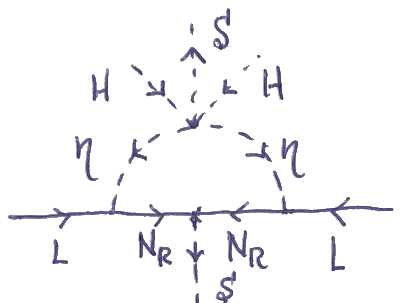
\includegraphics[scale=0.5]{rss}
  \caption{Radiative seesaw with small $\lambda_5$ (top $S$ can also be $S^{*}$ if required)}
  \label{fig:rss}
\end{figure}

The relevant Lagrangian must be consistent with
\begin{align}
  l+\eta=&n\,,& 2n=&s\,, & 2h=2\eta\pm s\,.
  % l+\eta=&n\,,& 2n=&s\,, & 2h=2\eta+s\,.
  % See:                            
\end{align}
The solution for minus sign in the last equation, corresponding to $S^*$ in the top part of figure~\ref{fig:rss}.,  with a global $\operatorname{U}(1)_{\text{global}}$~\cite{Suematsu:2017kcu}\footnote{Local by just adding $N_L$ with same charge $-1$} is displayed in table~\ref{tab:suematsu}.

\begin{table}
  \centering
  \begin{tabular}{c|ll}
    Fields&$\operatorname{U}(1)_{\text{global}}$& $\phantom{\operatorname{U}(1)_X}$\\ \hline
    $L$   & $l=\phantom{-}0$&$\phantom{l=-1}$\\
    $H$   & $h=\phantom{-}0$&$\phantom{h=-1-l=0}$\\
    $N_R$ & $n=-1$          &$\phantom{n=-1/2}$\\
    $\eta$& $\eta=-1$       &$\phantom{-1/2-l=1/2}$ \\
    $S$   & $s=-2$         &$\phantom{s=-1}$ \\
  \end{tabular}
  \caption{Global solution, see \url{./scotolocal.nb}, to diagram of charge flux in figure~\ref{fig:rss}}
  \label{tab:suematsu}
\end{table}

\end{document}
Therefore must include the fermion terms (matrix notation for family indices)
\begin{align}
  \mathcal{L}\supset h \left( N_R \right)^{\dagger} L \cdot \eta + y N_R N_R S + \text{h.c}\,.
\end{align}

After the spontaneous braking of the global symmetry we have the relevant terms
\begin{align}
  \mathcal{L}\supset \left[ h \left( N_R \right)^{\dagger} L \cdot \eta + M_R N_R N_R  +
  \widetilde{\lambda}_{5}\left(\eta^{\dagger} H\right)^{2}+\text { h.c } \right]
  +\mu_{2}^{2} \eta^{\dagger} \eta+\lambda_{3}\left(H^{\dagger} H\right)\left(\eta^{\dagger} \eta\right)+\lambda_{4}\left(H^{\dagger} \eta\right)\left(\eta^{\dagger} H\right),
\end{align}
where
\begin{align}
 M_R=& y \langle S \rangle\,,& \widetilde{\lambda}_5=&\lambda_5 \frac{\langle S \rangle }{M}\,.
\end{align}
If we assign zero lepton number to $N_R$ we can assign $0$ ($+1$)
lepton number to $\eta$ such that the term with coupling $h$
($\widetilde{\lambda}_5$) is violates lepton number. Therefore the
light neutrino masses are proportional to the product of
$y \widetilde{\lambda}_5$. In which follows we will drop the tilde in
$\lambda_5$.

The Lagrangian in the mass basis, relevant for the generation of neutrino masses is
\begin{align}
  \mathcal{L}\supset \frac{h}{\sqrt{2}} \left( N_R \right)^{\dagger} \nu_L \left( \rho^0+i A^0  \right)
  + M_R N_R N_R + \frac{1}{2}m_{\rho}^2 \rho^{02}+ \frac{1}{2}m_{A}^2 A^{02}\,.
\end{align}
which generate the two contribution to the neutrino mass displayed in figure~\ref{fig:massbas}

\begin{figure}
  \centering
  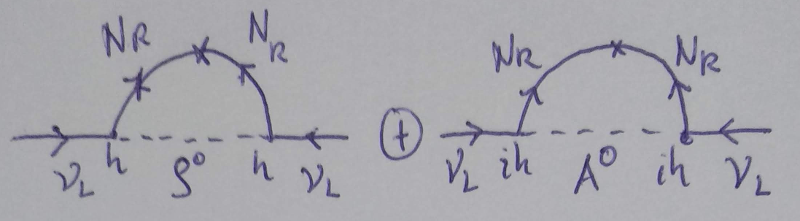
\includegraphics[scale=0.4]{massbas}
  \caption{Contribution to neutrino mass in mass basis}
  \label{fig:massbas}
\end{figure}

\begin{align}
 M^{\nu}_{ij}=&-\frac{h^2}{16\pi^2}M_R \left[ 
f \left( M_R^2,m_{\rho}^2 \right)-f \left( M_R^2,m_{A}^2 \right) \right].
\end{align}

\section{Singlet-doublet fermions with scalar singlets}
There~\cite{Restrepo:2015ura}

\begin{align}
  y_{i n\alpha}=&h_{i\alpha}N_{3n} 
\end{align}
and 
\begin{align}
   M^{\nu}_{ij}=&\sum_{\alpha}\frac{h_{i\alpha}h_{j\alpha}}{16\pi^2}\sum_{n=1}^3 \left( N_{3n} \right)^2m_{\chi_n}
\,f\left( m_{S_\alpha}^2,m_{\chi_n}^2 \right).
\end{align}

\subsection{Zee}

In the Zee model we can work in the Higgs-basis with $\left\langle H_1 \right\rangle=v/\sqrt{2}$,  $\left\langle H_2 \right\rangle=0$ \cite{AristizabalSierra:2006ri}. In that basis the scalar potential is
\begin{align}
  \label{eq:scalarpotentialinhiggsbas}
  V  = & \mu^{2}_{1}H_{1}^{\dagger}H_{1}
  + \mu^{2}_{2}H_{2}^{\dagger}H_{2}
  - [\mu^{2}_{3}H_{1}^{\dagger}H_{2} + \mbox{H.c.}]
  + \frac{1}{2}\lambda_{1}(H_{1}^{\dagger}H_{1})^{2}
  \nonumber\\
  & + \frac{1}{2}\lambda_{2}(H_{2}^{\dagger}H_{2})^{2}
  + \lambda_{3}(H_{1}^{\dagger}
  H_{1})(H_{2}^{\dagger}H_{2})
  + \lambda_{4}(H_{1}^{\dagger}
  H_{2})(H_{2}^{\dagger}H_{1})
  \nonumber\\
  & + \left\{
    \frac{1}{2}\lambda_{5}(H_{1}^{\dagger}H_{2})^{2}
    + [\lambda_{6}(H_{1}^{\dagger}H_{1})
    + \lambda_{7}(H_{2}^{\dagger}H_{2})]
    H_{1}^{\dagger}H_{2}
    +\mbox{H.c.}
  \right\}
  \nonumber\\
  & + \mu_{h}^{2}|h^{+}|^{2} + \lambda_{h}|h^{+}|^{4}
  + \lambda_{8}|h^{+}|^{2}H_{1}^{\dagger}H_{1} 
  + \lambda_{9}|h^{+}|^{2}H_{2}^{\dagger}H_{2}
  \nonumber\\
  & + \lambda_{10}|h^{+}|^{2}(H_{1}^\dagger H_{2}
  + \mbox{H.c.})
  + \mu\epsilon_{\alpha\beta}H_{1}^{\alpha}
  H_{2}^{\beta}h^{-}.
\end{align}

We define
\begin{align}
  H_1=&
  \begin{pmatrix}
    G^{+}\\
    \operatorname{Re}\left( H_1^{0} \right)+i G^{0}/\sqrt{2}\\
  \end{pmatrix}&
  H_2=&
  \begin{pmatrix}
    H^{+}\\
    \operatorname{Re}\left( H_2^{0} \right)+i A^{0}/\sqrt{2}\\
  \end{pmatrix}
\end{align}
The minimum equations come from
\begin{align}
  \frac{\partial V}{\partial \operatorname{Re}\left( H_1^{0} \right)}=&
\frac{\partial }{\partial \operatorname{Re}\left( H_1^{0} \right)} \left[ 
\mu^{2}_{1}\left(\operatorname{Re}H_{1}^{0}  \right)^2
+\frac{1}{2}\lambda_1 \left(\operatorname{Re}H_{1}^{0}  \right)^4+\cdots  \right]\nonumber\\
=&2\mu^{2}_{1}\operatorname{Re}H_{1}^{0}  
+\frac{1}{2}\lambda_1 4 \left(\operatorname{Re}H_{1}^{0}  \right)^3+\cdots
\end{align}

\begin{align}
  \frac{\partial V}{\partial \operatorname{Re}\left( H_2^{0} \right)}=&
-\mu^2_32\operatorname{Re}H_1^0+\lambda_6 2  \left(\operatorname{Re}H_1^0 \right)^3+\cdots
\end{align}

From the conditions
\begin{align}
  \left.   \frac{\partial V}{\partial \operatorname{Re}\left( H_{1,2}^{0} \right)} \right|_{\left\langle H_1  \right\rangle \to v/\sqrt{2},\left\langle H_2  \right\rangle \to 0}=&0\,,
\end{align}
we have
\begin{align}
  \mu_1^2+\frac{1}{2} \lambda_1 =&0 &-\mu_3+\frac{1}{2}\lambda_6=&0
\end{align}
or
\begin{align}
   \mu_1^2=&-\frac{1}{2} \lambda_1  &\mu_3=&\frac{1}{2}\lambda_6\,.
\end{align}
Replacing back in the potential, we have for the charged scalars that
In the basis $\mathbf{\Phi}^{\dagger}=(G^{-}, 
H^{-}, h^{-})$ 
the squared-mass matrix for the charged Higgs states is given by
\begin{align}
  \label{eq:scalarM}
\mathcal{L}_{\text{charged}}= \boldsymbol{\Phi}^{\dagger} {\cal M}_{C}^{2}\boldsymbol{\Phi}+\cdots\;,
\end{align}
where 
\begin{align}
  {\cal M}_{C}^{2}=&
  \begin{pmatrix}
    0   &          0         &  0                   \\
    0   &  M_{H^{\pm}}^{2}   &  -\mu v/\sqrt{2}     \\
    0       &  -\mu v/\sqrt{2} &  {\cal M}_{33}^{2}   
  \end{pmatrix},
and
\end{align}
\begin{align}
  \label{eq:entriesofmassmatrix}
  M_{H^{\pm}}^{2} =& \mu_{2}^{2} +\frac{1}{2}v^{2}\lambda_{3}
  \nonumber\\
  {\cal M}_{33}^{2} =& \mu_{h}^{2} + v^{2}\lambda_{8}\,.
\end{align}
By defining the mass basis state as $\mathbf{S}=\left( G^-,h_1^.,h_2^- \right)$, then after the rotation
\begin{align}
\mathbf{S}=R \boldsymbol{\Phi}\,,
\end{align}
where
\begin{align}
    \label{eq:rotationM}
  R =& 
  \begin{pmatrix}
    1 &      0       &     0       \\
    0 & \cos\varphi  &  \sin\varphi\\
    0 & -\sin\varphi &  \cos\varphi
  \end{pmatrix}&\,.
\end{align}
Then,
\begin{align}
  \mathcal{L}_{\text{charged}}=M_1^2 h_1^+ h_1^-
+M_2^2 h_2^+ h_2^-+\cdots
\end{align}
The relevant terms for neutrino masses in the mass eigenstate basis reads
\begin{align}
  \mathcal{L}_{\nu}=&
\Pi'_2\cos\varphi \left( e_R \right)^{\dagger}\nu_L h_1^-
-\Pi'_2\sin\varphi \left( e_R \right)^{\dagger}\nu_L h_2^-
+f_{ji} \left( e_L \right)_j\left(\nu_L  \right)_i  \sin\varphi h_1^{+}
+f_{ji} \left( e_L \right)_j\left(\nu_L  \right)_i  \cos\varphi h_2^{+} \nonumber\\
&+\widehat{M}_l \left( e_R \right)^{\dagger}e_L+\text{h.c}
+M_1^2 h_1^+ h_1^-
+M_2^2 h_2^+ h_2^-
\end{align}
Therefore
\begin{align}
  M_{ij}^{\nu}\propto 
\left( \Pi'_2 \right)_{ik}\cos\varphi \widehat{M}_{kk} f_{jk}\sin\varphi
\end{align}




In that case $n$ corresponds to the usual leptons labeled with $i,j,k,\ldots$, and $\alpha=1,2$

\begin{align}
  \mathcal{L}=&\overline{\nu_{Lj}}O_{jk}e_{Rk}R_{1\alpha}h_{\alpha}^{+}+ \nonumber\\
              &{\nu_{Li}}^{\text{T}}C \left( 2 f_{ik} \right)e_{Lk}R_{2\alpha}h_{\alpha}^{+}+\nonumber\\
              &m_k  \overline{e_{Lk}} e_{Rk}+\text{h.c}\,,
\end{align}
Therefore

\begin{align}
  y_{i k\alpha}=&O_{i k}R_{1\alpha} \nonumber\\
  y_{j k\alpha}=&2f_{i k}R_{\alpha 1} \nonumber\\
\end{align}
where
\begin{align}
  \mathbf{R}=
  \begin{pmatrix}
    \cos\varphi & -\sin\varphi\\
    \sin\varphi & \cos\varphi\\    
  \end{pmatrix}
\end{align}
\begin{align}
  M^{\nu}_{ij}=&-\sum_k \sum_{\alpha}
\frac{2O_{ik}R_{1\alpha}f_{jk} R_{2\alpha}}{16\pi^2}m_{k}\left[ \operatorname{cte}(\infty)+
f \left( m_{\chi_n}^2,m_{S_{\alpha}}^2 \right) \right] \nonumber\\
=&-\sum_k 
\frac{O_{ik}f_{jk} }{8\pi^2}m_{k}\left[ R_{11}R_{21}\operatorname{cte}(\infty)+
R_{11}R_{21}f \left( m_k^2,M_1^2 \right)
+R_{12}R_{22}\operatorname{cte}(\infty)+
R_{12}R_{22}f \left( m_k^2,M_2^2 \right) \right] \nonumber\\
=&-\sum_k \frac{O_{ik}f_{jk} }{8\pi^2}m_{k}\cos\varphi\sin\varphi
\left[f \left( m_k^2,M_1^2 \right)-f \left(m_k^2,M_2^2 \right) \right] \nonumber\\
\approx&-\sum_k \frac{O_{ik}f_{jk} }{16\pi^2}m_{k}\sin 2\varphi
\left[f \left( 0,M_1^2 \right)-f \left(0,M_2^2 \right) \right] \nonumber\\
=&-\sum_k \frac{O_{ik}f_{jk} }{16\pi^2}m_{k}\sin2\varphi
\left[\frac{M_1^2M_2^2\ln \left(M_1^2\right)-M_1^2M_2^2\ln \left(M_2^2\right)}{M_1^2M_2^2} \right] \nonumber\\
=&\sum_k \frac{f_{jk}m_kO_{ik} \sin2\varphi }{(4\pi)^2}
\ln \left( \frac{M_2^2}{M_1^2}\right),
\end{align}
To compare with \cite{AristizabalSierra:2006ri}. There is factor 2?
\begin{align}
  M^{\nu}_{ij} =&-\frac{\sin2\varphi}{\left(4\pi\right)^2}\sum_k \left( f_{ik}m_kO_{jk} +f_{jk}m_kO_{ik} \right)
\left[f \left( m_k^2,M_1^2 \right)-f \left(m_k^2,M_2^2 \right) \right]
\end{align}
In the generic basis, The important factor is
\begin{align}
\label{eq:gz}
  f_{ik}m_kO_{jk} +f_{jk}m_kO_{ik}=&
f_{ik}m_k \left(  -\sqrt{2}\frac{\tan\beta}{v}m_k+\frac{1}{\cos\beta}{\Pi_2}_{jk} \right)
+f_{jk}m_k\left( -\sqrt{2}\frac{\tan\beta}{v}m_k+\frac{1}{\cos\beta}{\Pi_2}_{ik} \right) \nonumber\\
=&
-\sqrt{2}\frac{\tan\beta}{v}\left(f_{ik}m_k^2+m_k^2f_{jk}\right)
 +\frac{1}{\cos\beta}\left(  f_{ik}m_k{\Pi_2}_{jk}+{\Pi_2}_{ik}m_kf_{jk} \right)
\end{align}
Seem to be that there is a mistake in \cite{hep-ph/0307172}w wiht $\tan\beta$.
\subsection{Minimal Zee}
According to \cite{hep-ph/0307172}, the famous Zee-Wolfenstein matrix by settin $\Pi_2=0$ in eq.~\eqref{eq:gz}


This case corresponds to the limit $\Pi_2=0$ of ~\cite{AristizabalSierra:2006ri}

\begin{align}
  \mathcal{L}=&-\sqrt{2}\frac{\tan\beta}{v}\overline{\nu_{Lj}}m_j e_{Rj}R_{1\alpha}h_{\alpha}^{+}+ \nonumber\\
              &{\nu_{Li}}^{\text{T}}C \left( 2 f_{ik} \right)e_{Lk}R_{2\alpha}h_{\alpha}^{+}+\text{h.c}\,,
\end{align}
Therefore

\begin{align}
  y_{i k\alpha}=& -\sqrt{2}\frac{\tan\beta}{v}m_k \delta_{ik}R_{1\alpha} \nonumber\\
  y_{j k\alpha}=&2f_{i k}R_{\alpha 1} \nonumber\\
\end{align}

\begin{align}
  M^{\nu}_{ij}
=&\sum_k \frac{f_{jk}m_k \delta_{ik} \sin2\varphi }{(4\pi)^2}
\ln \left( \frac{M_2^2}{M_1^2}\right) \nonumber\\
=& \frac{f_{ji}m_i\sin2\varphi }{(4\pi)^2}
\ln \left( \frac{M_2^2}{M_1^2}\right).
\end{align}
which is non-zero only for $i\ne j$.

%%% Local Variables: 
%%% mode: latex
%%% TeX-master: "beyond"
%%% End: